%% ----------------------------------------------------------------------------
% BIWI SA/MA thesis template
%
% Created 09/29/2006 by Andreas Ess
% Extended 13/02/2009 by Jan Lesniak - jlesniak@vision.ee.ethz.ch
%% ----------------------------------------------------------------------------
\newpage
\chapter{Experiments and Results}
\label{sec:experimentsandresults}
Describe the evaluation you did in a way, such that an independent researcher can repeat it. Cover the following questions:
\begin{itemize}
    \item \textit{What is the experimental setup and methodology?} Describe the setting of the experiments and give all the parameters in detail which you have used. Give a detailed account of how the experiment was conducted.
    \item \textit{What are your results?} In this section, a \emph{clear description} of the results is given. If you produced lots of data, include only representative data here and put all results into the appendix.
\end{itemize}

\section{Training Models on MNIST, CIFAR and fastMRI}
In order to explore hyperparameters of the model architecture and debug the implementation it was decided to first train models on datasets considered trainable with less compute time. Two very well known datasets in computer vision that use low-resolution images are CIFAR10 and MNIST.~\autocite{cifar,mnist}
\begin{figure}[h]
    \centering
    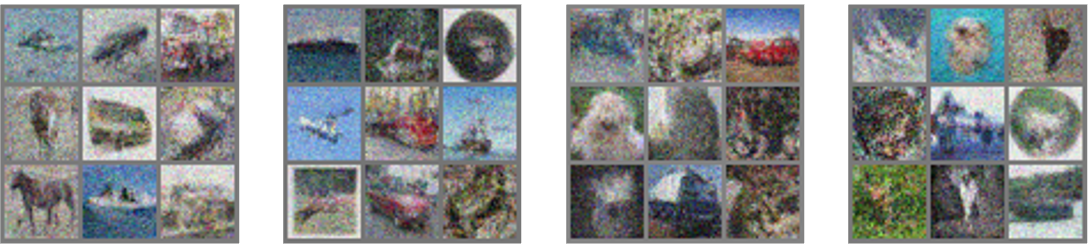
\includegraphics[width=.75\textwidth]{images/cifarsamples.png}
    \caption[Samples generated from CIFAR10]{Samples from the best performing model trained on CIFAR10 using a linear schedule: While the variance in the samples is large, suggesting that the model is able to capture the whole distribution, the samples are not completely denoised and therefore sample quality is seriously degenerated. As can be seen later, this was not observed when training on datasets where the image resolution was higher.}
    \label{fig:cifarsamples}
\end{figure}

\begin{figure}[h]
    \centering
    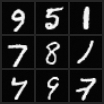
\includegraphics[width=.15\textwidth]{images/mnistsamples.png}
    \caption[Samples generated from MNIST]{Samples from the best performing model trained on MNIST}
    \label{fig:mnistsamples}
\end{figure}

Unconditional sampling was performed in order to verify the sample quality and whether the model was able to capture the main modes of the training data distribution. For a quantitative analysis of sample quality and mode coverage/log-likelihood of trained models Nichol et al. use FID score and Monte-Carlo log-likelihood estimates. FID requires the training of an additional classifier network, which only makes sense on standardized datasets with class labels such as ImageNet or CIFAR.~\autocite{imagenet, cifar} Pretrained classifiers are available for these datasets, which makes scores comparable among different generative models. The fastMRI dataset is not meant for classification tasks, therefore
\begin{figure}[h]
    \centering
    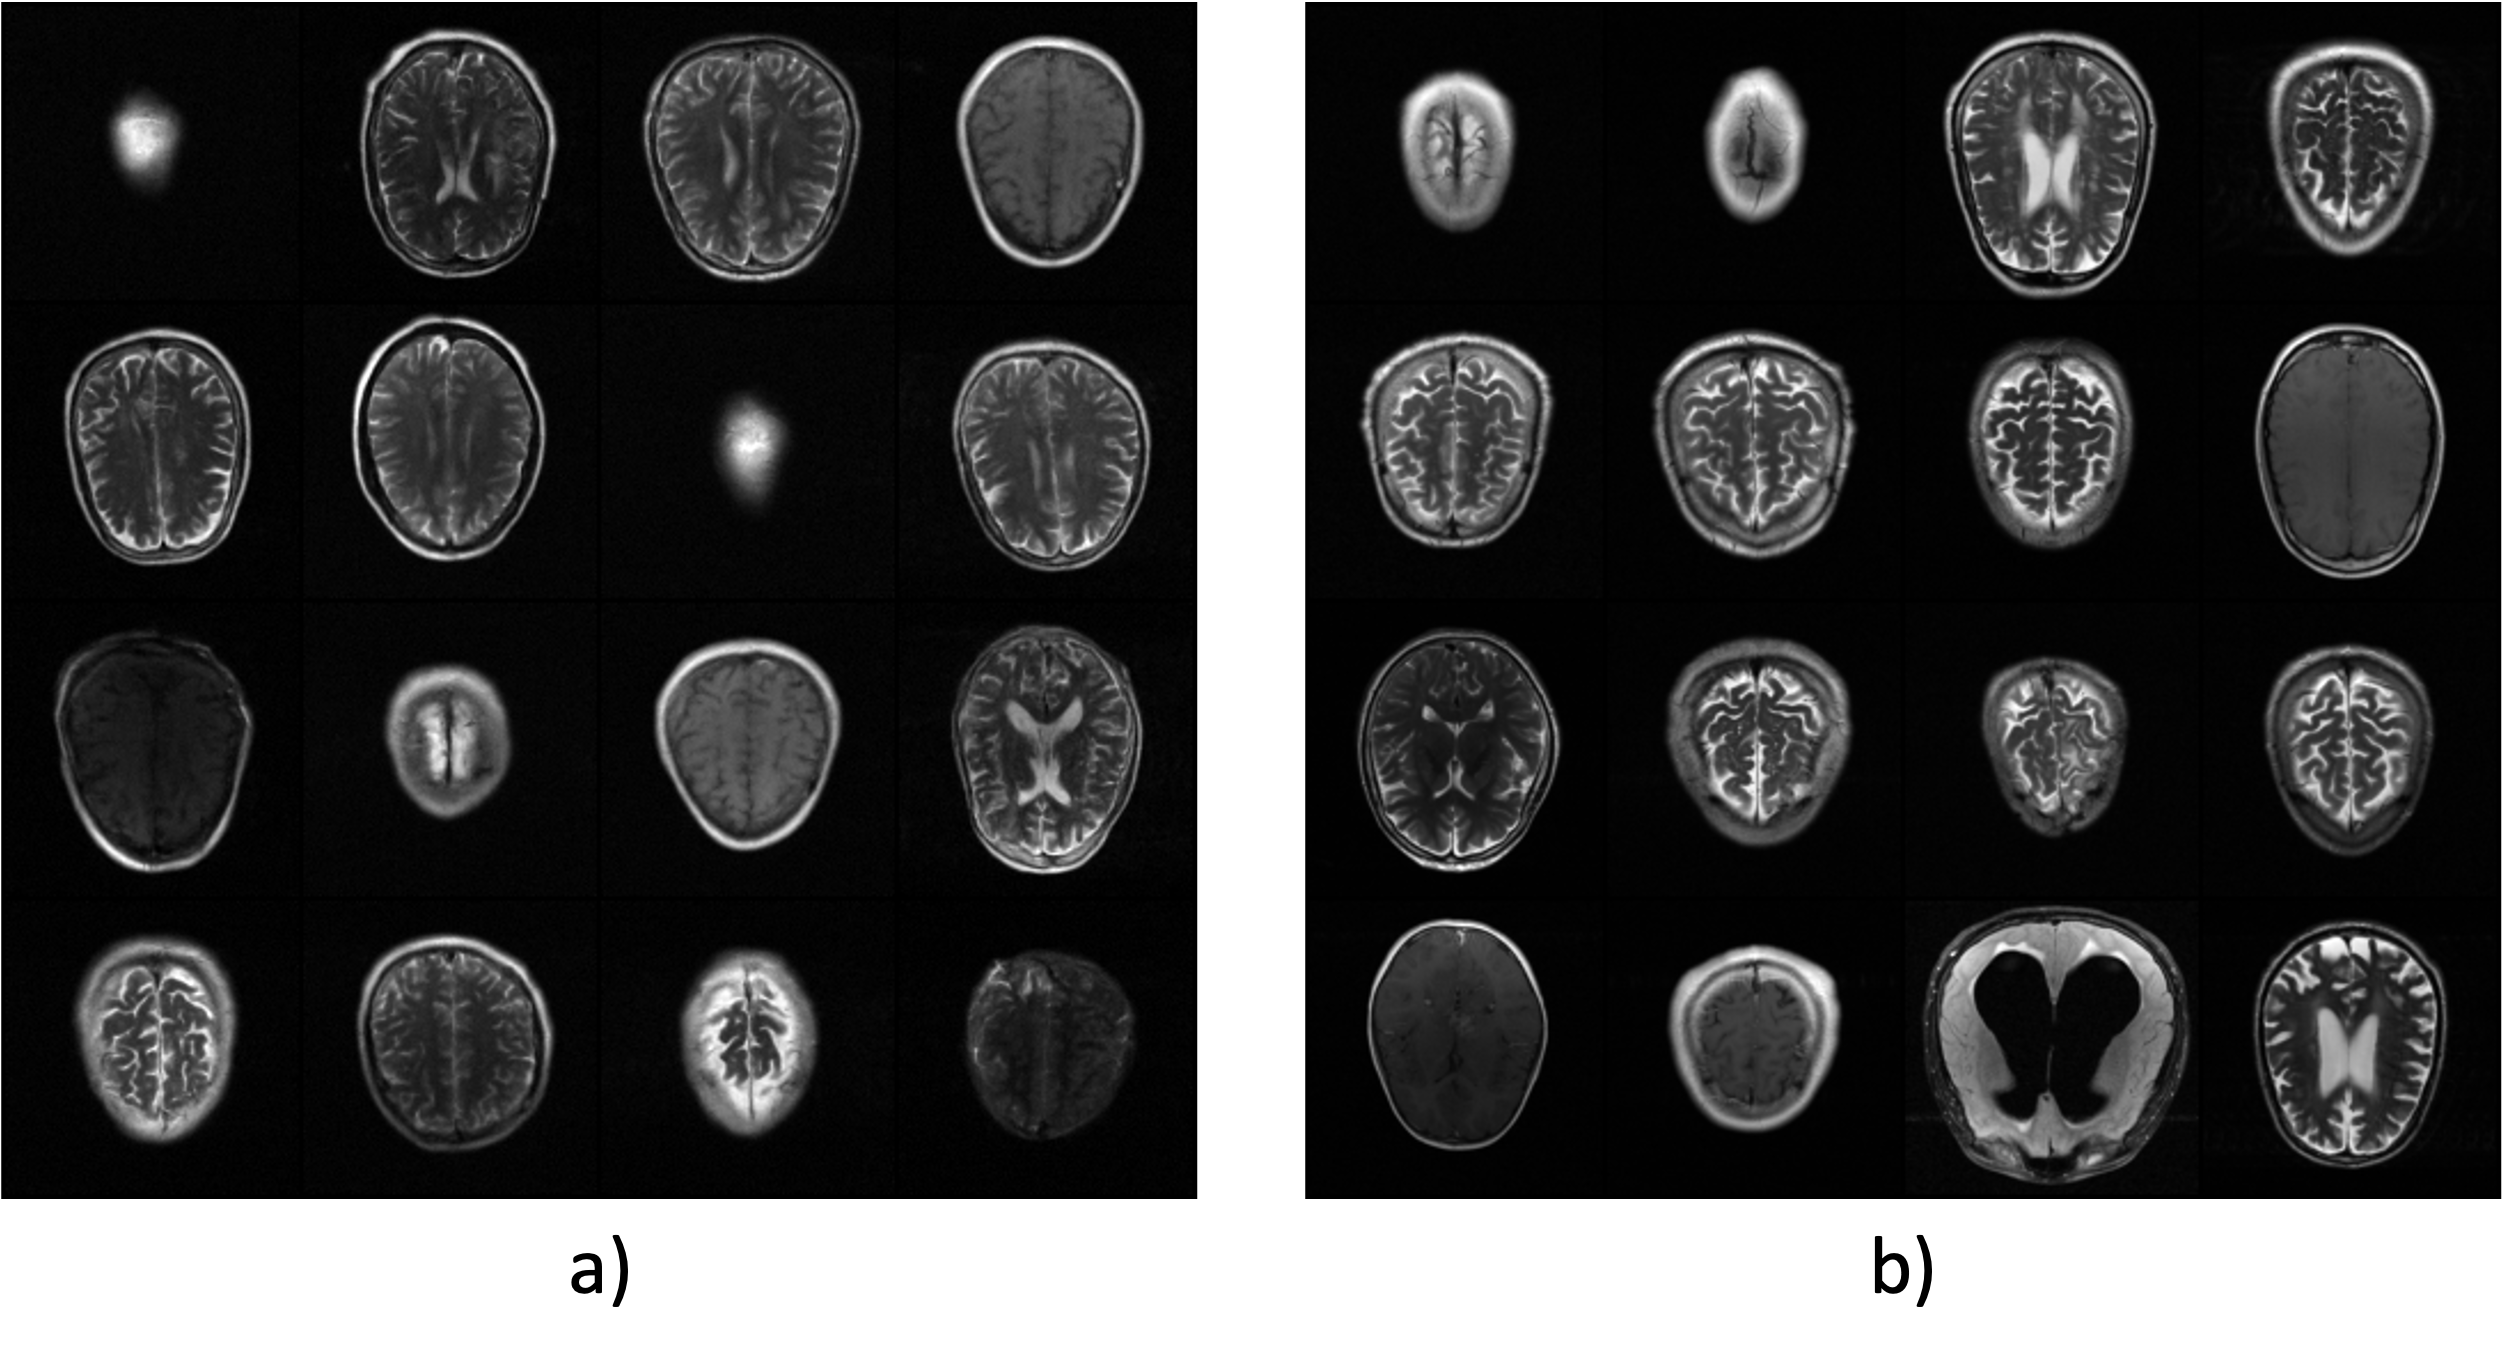
\includegraphics[width=.66\textwidth]{images/samples_unconditional.png}
    \caption[Samples from Data Set and Unconditional Sampling]{a) Unconditionally sampled examples, produced by the best-performing model; b) Examples from the training data set (fastMRI, RSS reconstruction); As can be seen, sample quality is comparable to the quality of the training samples and the variability among the samples is high, indicating a decent log-likelihood and mode coverage of the model.}
    \label{fig:uncondsampling}
\end{figure}

\subsection{Influence of Schedules and Image Size on the Forward Diffusion}
\label{sec:forward_diff_experiments}
Ho et al. had derived a closed form solution to the forward process of DDPMs and Nichol et al. investigated alternative options for the noise scheduling.~\autocite{ho2020denoising,nichol2021improved} They concluded that the important parameters to model are not the variances $\beta$ of the transitions, but the variances $1-\bar{\alpha}$ of the closed-form forward process, since they are the ones responsible for the destruction of information.

They decided to go with a squared cosine function, since this would be close to linear smooth out towards the critical beginning and end points of the process. In Fig.\ref{fig:alphadash} you can see how $1-\bar{\alpha}$ and $\beta$ behave for both approaches. It is immediately visible that the variances reach the maximum too early and flatten out for the linear schedule. This leads to the intuition that the last few steps are not very useful.

\begin{figure}[h]
    \centering
    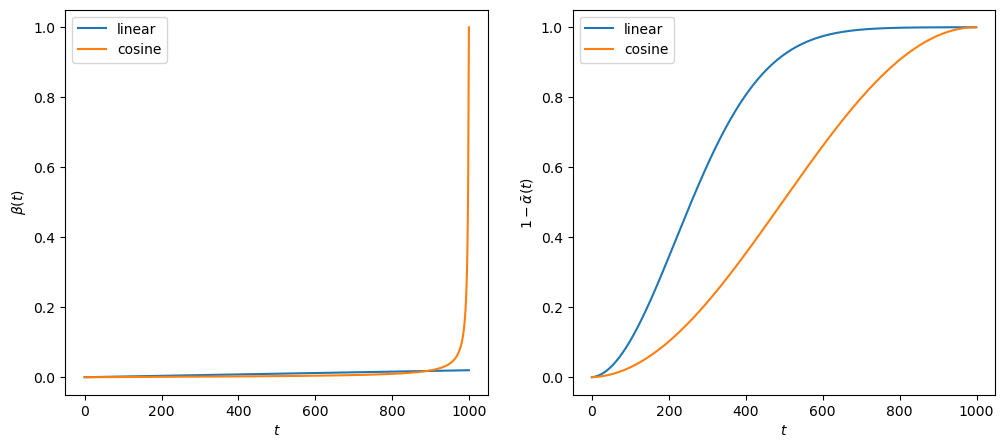
\includegraphics[width=.5\textwidth]{images/variance_schedule_alphadash.png}
    \caption{Variance Schedule Approaches: Modeling the $1-\bar{\alpha}$ as an approximate linear function (right cosine) and deriving $\beta$ (left cosine), or modeling $\beta$ as a linear function (left linear) and deriving $1-\bar{\alpha}$.}
    \label{fig:alphadash}
\end{figure}

The intution can experimentally confirmed by measuring how closely we get to isotropic noise when passing samples through the forward process. For this a batch of 50 times the same image was passed through the different steps of the process and the covariance matrix was calculated. As a metric for how close the covariance matrix was to the identity covariance matrix of pure i.i.d Gaussian noise, the identity matrix was subtracted and the mean of the absolute value of the matrix calculated. The results can be seen in Fig.~\ref{fig:noisecloseness} and confirm the intuition: When using linear scheduling we reach the closest point to pure noise already after around 600 steps for small images, and after around 700 for larger images. Cosine scheduling also performs worse on smaller images than on larger ones, but is still capable providing value for at least 850 timesteps.

\begin{figure}[h]
    \centering
    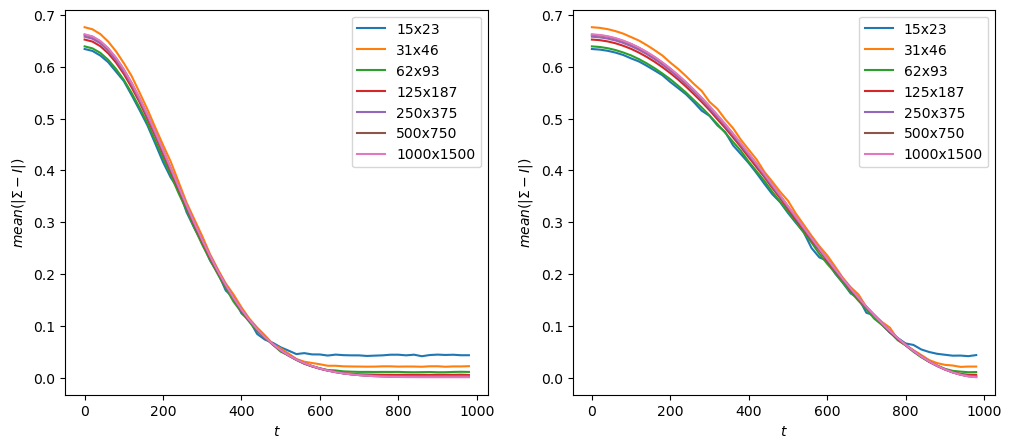
\includegraphics[width=.5\textwidth]{images/frobenius_norm.png}
    \caption{Closeness to noise for linear scheduling (left) and cosine scheduling (right).}
    \label{fig:noisecloseness}
\end{figure}

\section{Image Inpainting \& Low-Frequency Guidance}
The works by Lugmayr et al.~\autocite{lugmayr2022repaint} and Choi et al.~\autocite{choi2021ilvr} were the main motivation to pursue an approach of conditioning unconditionally trained DDPMs. As a first step it was therefore important to recreate their results before adapting them to the task of undersampled MRI. The update steps of the reverse diffusion process were formulated according to~\ref{sec:freqreplacement} and the results can be seen in Fig.~\ref{fig:repaint} and Fig.~\ref{fig:ilvr}. Using Lugmayr et al.'s suggested hyperparameters for resampling (jump length of 10, with 10 resamplings) was indeed observed to help with creating semantically meaningful reconstructions with the exception of one of the sample images (lowest row, second from left), but this specific sample also caused issues with ILVR, suggesting that the distributional mode of that image type was not learned well by the model. Since it is an unusual type of image, it was likely not represented well in the training data.
\begin{figure}[h]
    \centering
    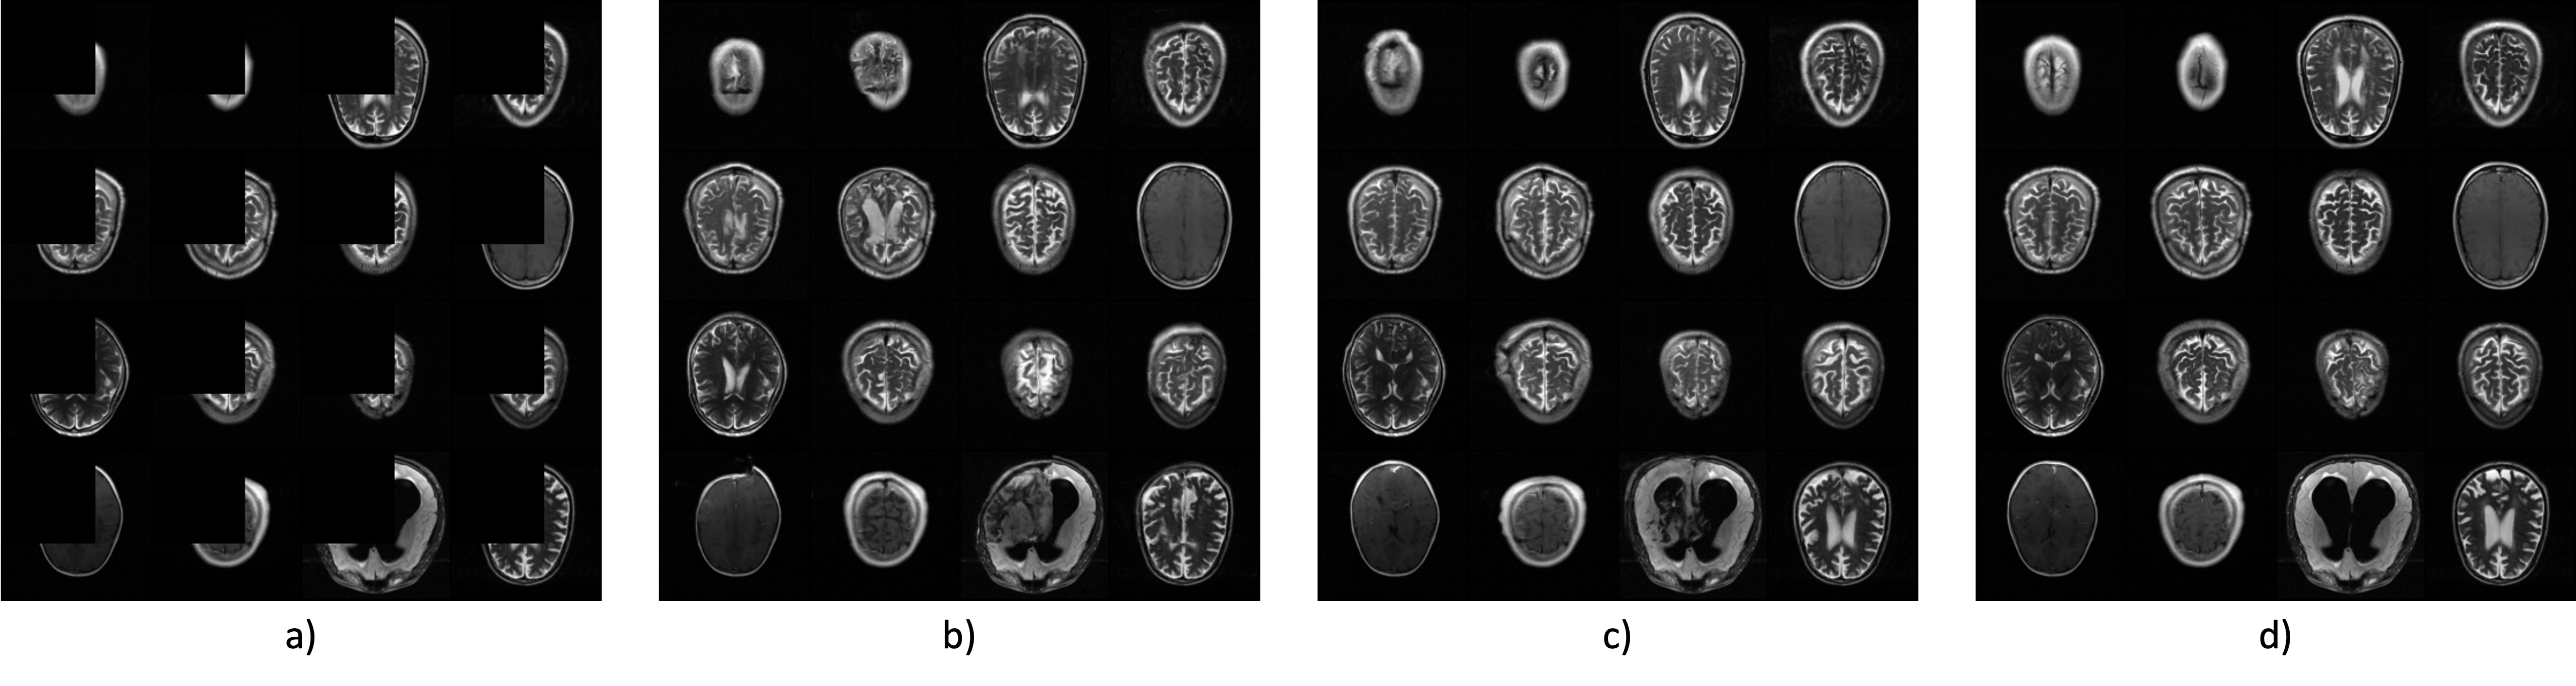
\includegraphics[width=.8\textwidth]{images/repaint.png}
    \caption[Inpainting and Resampling]{Inpainting and Resampling: a) Masked images used for the RePaint-style conditioning of the unconditional DDPM. b) Results from direct sampling. The reconstructed areas are often semantically wrong. c) Results from sampling with resampling with jump length $j=10$ and resamplings $r=10$ as suggested by Lugmayrs et al~\autocite{lugmayr2022repaint}. As observed in their work, the resampling strategy helps with semantically meaningful reconstruction. d) Ground truth images for comparison.}
    \label{fig:repaint}
\end{figure}

\begin{figure}[h]
    \centering
    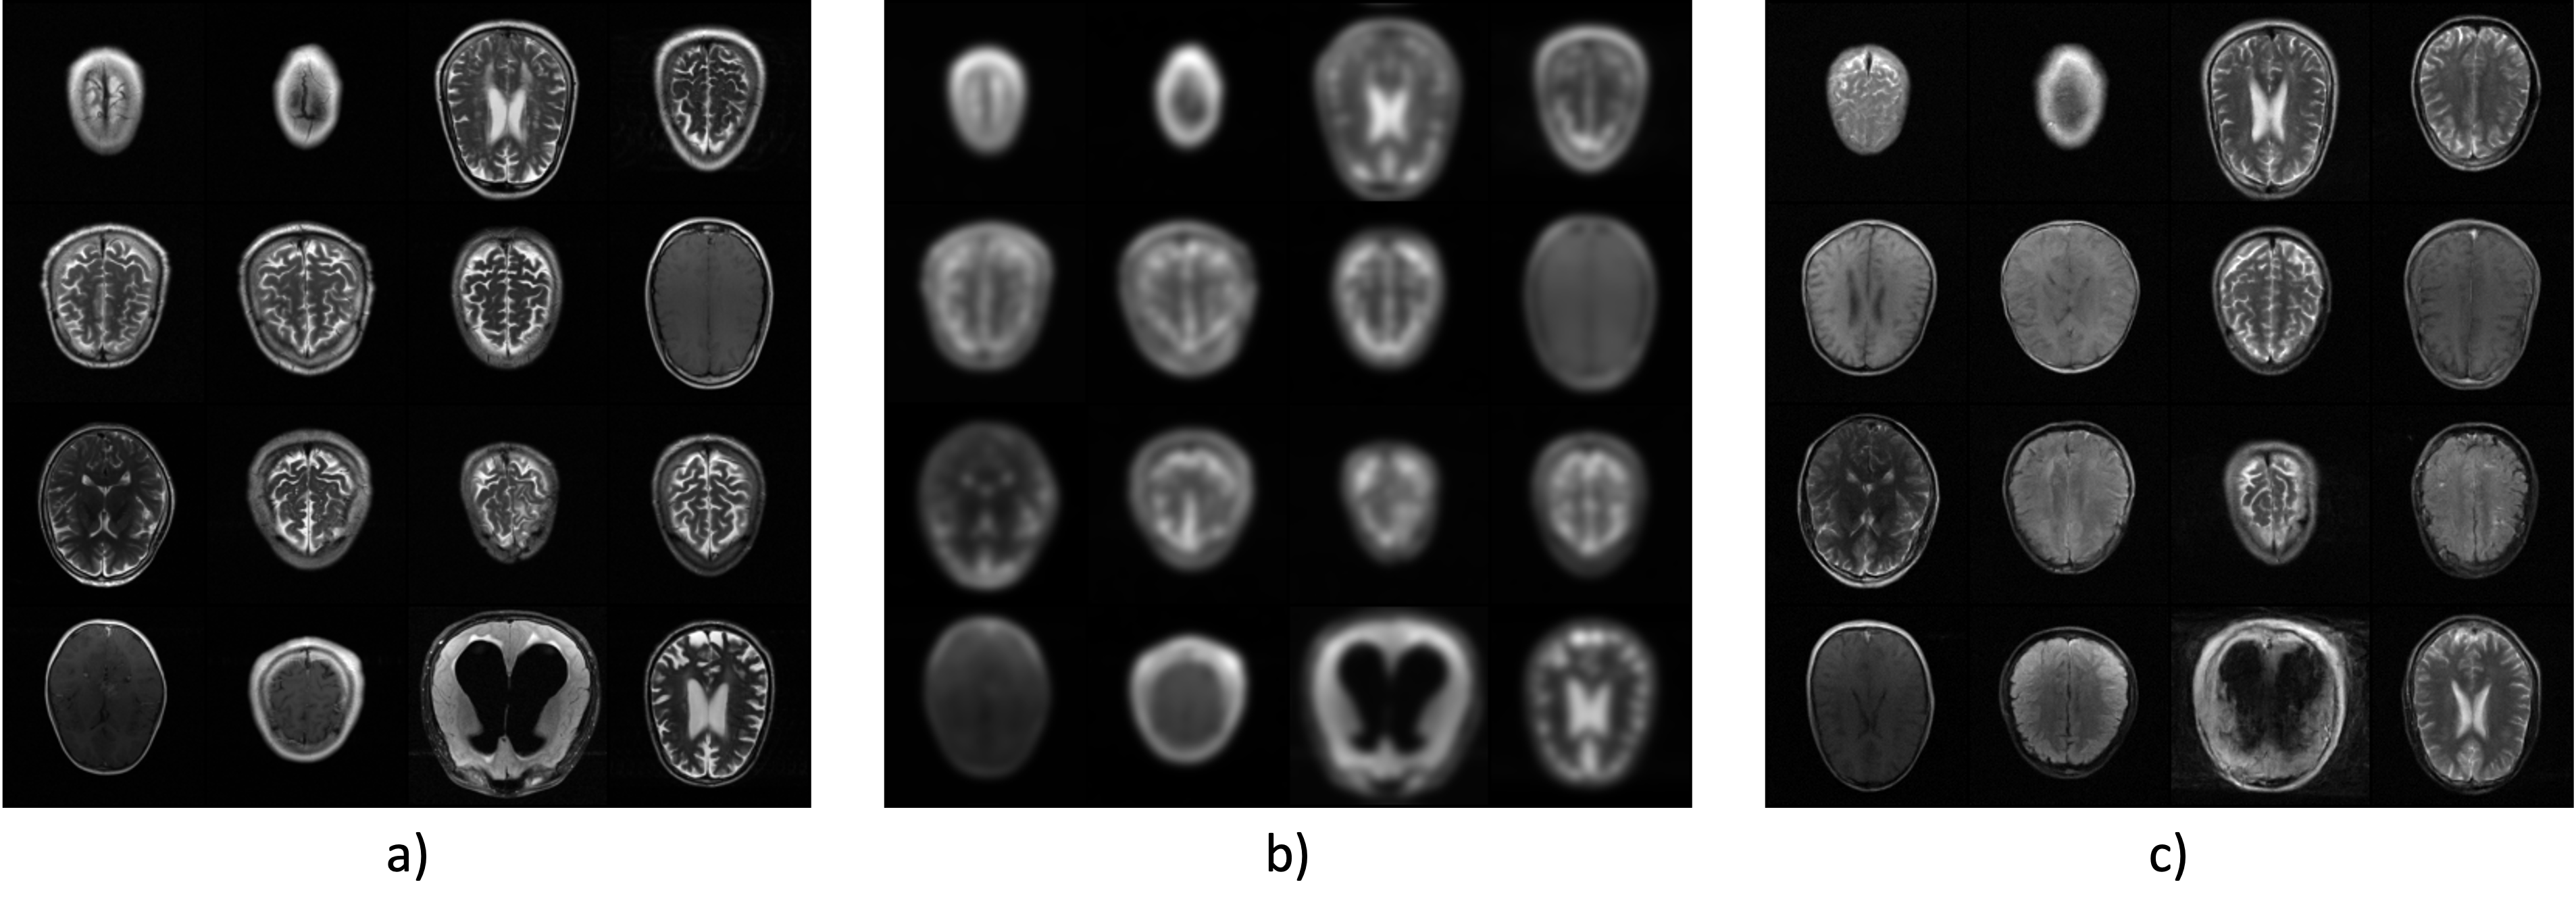
\includegraphics[width=.6\textwidth]{images/ilvr.png}
    \caption[ILVR -- Low-Frequency Guidance]{ILVR -- Low-Frequency Guidance: a) Shows the original guidance images, b) the filtered version used for guidance and c) the final predictions using this guidance. As can be seen, the predictions are of good perceptual quality, but the predictions often do not match the ground truth images, indicating that the filtering was too strong in this specific case.}
    \label{fig:ilvr}
\end{figure}

\section{Masked K-Space Substitution}
Lugmayr et al. use unconditional DDPMs to perform inpainting, which is a similar task to the reconstruction of undersampled MRI and are particularly successful by using resampling. This resampling process gives the network more time to create a globally semantically meaningful image.~\autocite{lugmayr2022repaint} Choi et al. replace low frequencies of the prediction with low frequencies of the latent representation of a target image to condition the diffusion process.~\autocite{choi2021ilvr} Since undersampled MRI still always contains global information, it was not expected, that resampling would have the same effect as with Lugmayr et al., nevertheless it was expected to be an option for better sample fidelity through additional computation cost. The implementation follows below equation, where both, the latent prediction $x_t$ is Fourier-transformed and the predicted frequencies are replaced with known ones from $s_t$ by the masking operation $\mathcal{M}$.
\begin{equation}
    x_{t-1} = x_t - \mathcal{F}^{-1}\left(\mathcal{M}\circ\mathcal{F}(x_t) + \mathcal{M}(s_t)\right)
\end{equation}
As mentioned in~\ref{sec:freqreplacement}, $s_t$ can be derived by applying noise either in the image space or directly in k-space and the results using both techniques are depicted in Fig.~\ref{fig:freqreplacement}. Reconstruction quality is far from great, especially for the low acceleration of factor $\approx 4.12$ with noticeable aliasing artifacts and unsharp edges, which might stem from the fact that the mask is essentially a box filter with multiple passbands and might therefore induce ringing artifacts. Aliasing and ringing are usually evaded by a better filter choice and the simplest choice of filter that avoids these artifacts is a Gaussian. Gaussian filters are also linear filters, which means that they integrate well into the framework introduced in~\ref{sec:freqreplacement}. The downside of applying a Gaussian filter is, that the sampled higher frequencies would be discarded, which would not only be wasteful, but the results in Fig.~\ref{fig:ilvr} showed that they are likely important for guidance. The next section will explore the idea of adding information gradually over the reverse diffusion process in order to give the model more time for reconstruction and to avoid frequency mismatch during the process that leads to artifacts.
\begin{figure}
    \centering
    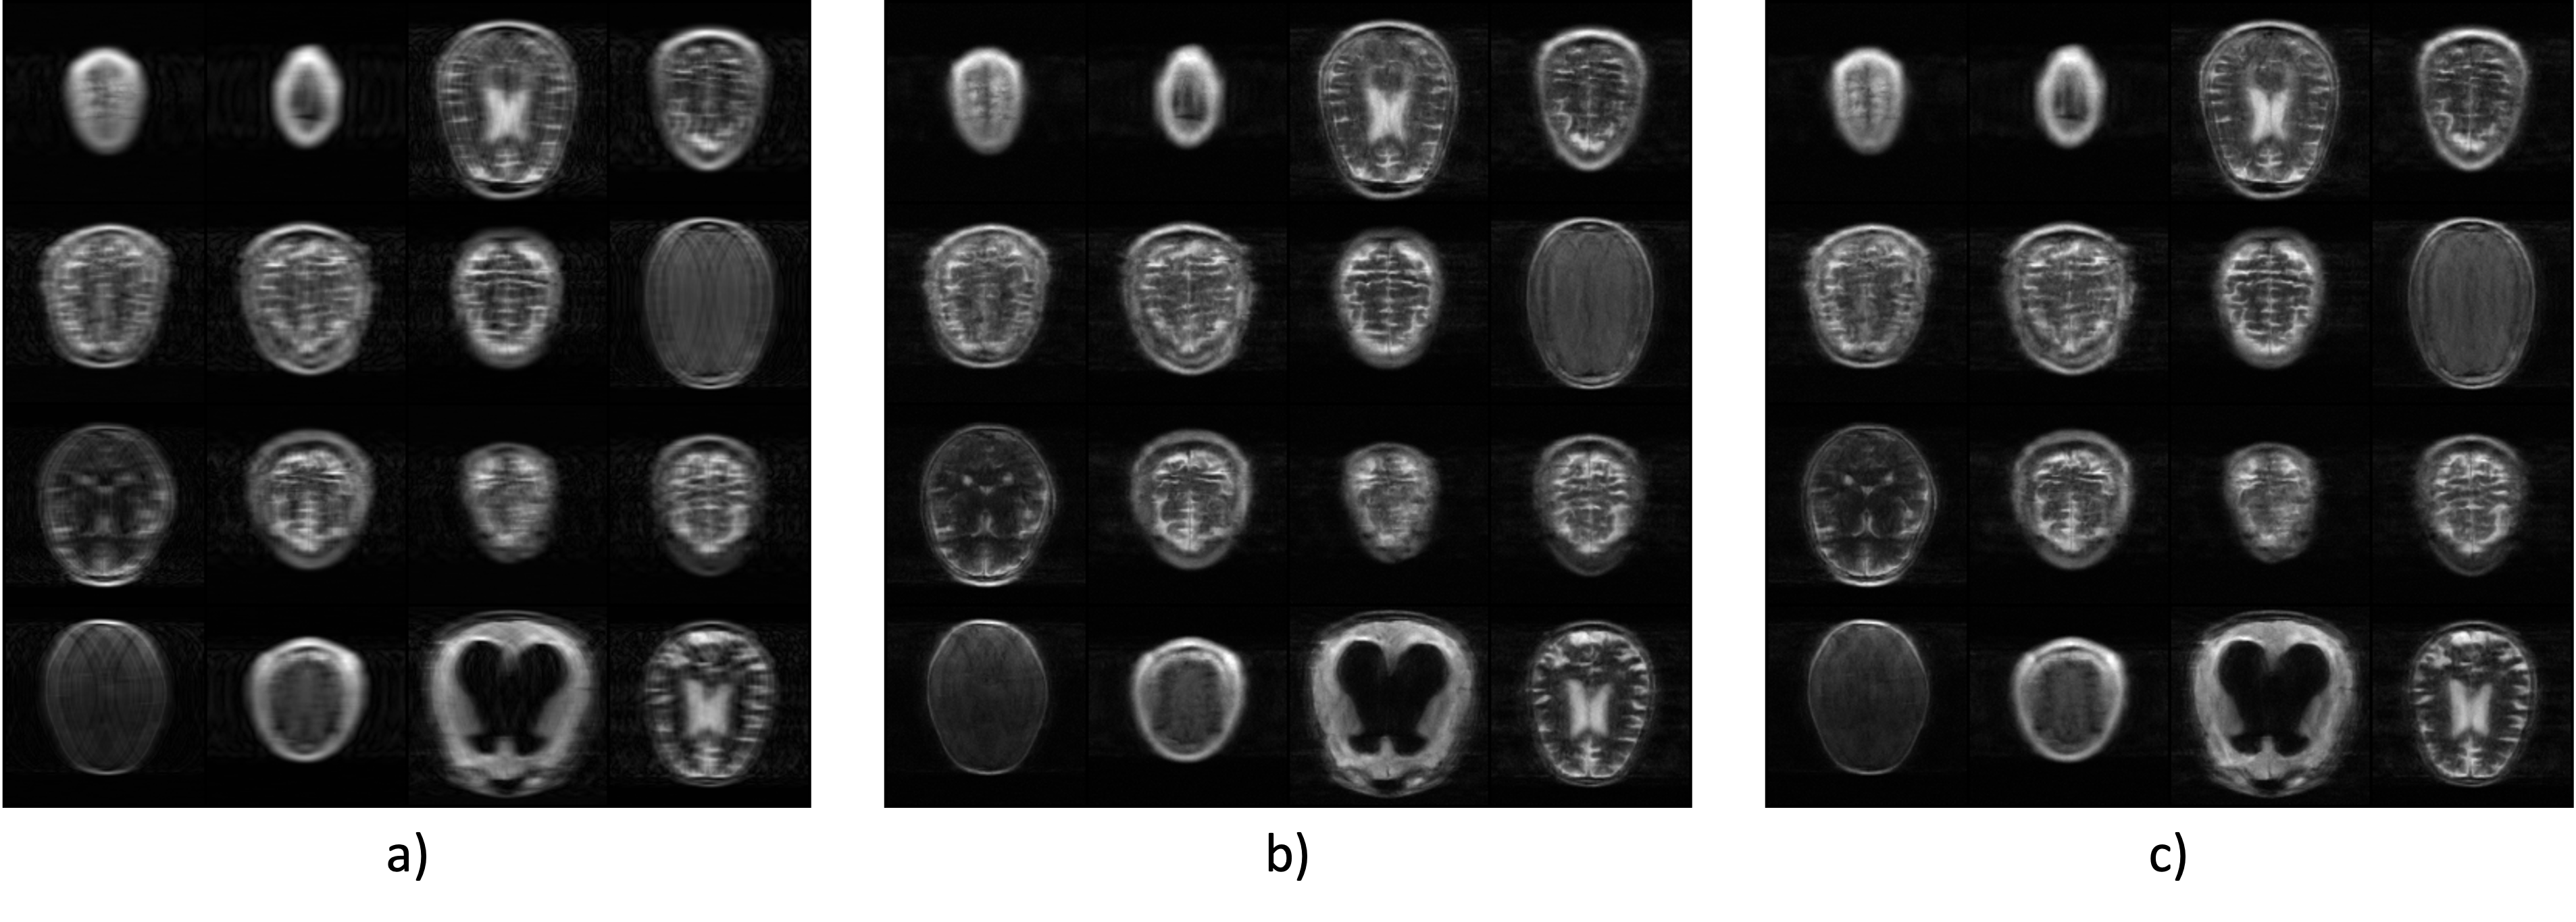
\includegraphics[width=.6\textwidth]{images/freq_replacement.png}
    \caption[Frequency Replacement]{Diffusion guidance using frequency replacement: a) Corrupted samples from an acceleration $\approx 4.12$. b) Results from applying noise directly on k-space (see~\ref{sec:freqreplacement}). c) Results from applying noise in the image space. The reconstruction quality is similar in both cases, but significantly worse than experiments with RePaint and ILVR from the previous section would suggest. The reconstructions show aliasing artifacts and possibly ringing artifacts at the edges, which indicate serious frequency mismatch.}
    \label{fig:freqreplacement}
\end{figure}


\section{Variance in Predictions and Filtered Diffusion}
\label{sec:predvariance}
Aliasing arises from mismatches between predicted and introduced frequency information. Aliasing can be avoided by using low-pass filters, but the k-space mask is specifically sampled such that it also contains some information from higher frequencies. Naive low-pass filtering would make this information inaccessible and the sampling of those frequencies useless. Since the SNR (signal-to-noise-ratio) in natural images is much higher in the lower frequencies than in the lower ones, it was hypothesized that it might be possible to add frequency information gradually during the denoising process in order to avoid aliasing, lower frequencies first and higher ones only towards the end.

In order to empirically study this hypothesis, a single sample was denoised and its latent representations at every 10th timestep were saved. These latent representations were copied into batches of 100 equal latent representations and the denoising process was continued for all these batches. Fig.~\ref{fig:predvariance} shows 4 of these samples for a subset of starting points. As can be seen, when starting from $t\geq700$, the samples still have a lot of variability and share very few common features. When starting later in the process, the samples clearly stem from the same distributional mode and only differ in the details. Since high frequencies are responsible for carrying information on details, this supports the hypothesis, but it becomes more evident, when looking at the variances of the spectral representations as seen in Fig.~\ref{fig:spectralvariance}. The variances were estimated over the frequency representations of all the final predictions in a batch (100 samples, denoised from $t$) and high variance means that this frequency was not yet determined at that specific $t$. As can be clearly seen in the figure, the variance is concentrated in the low frequencies when starting at larget $t$, and the variance in the low frequencies increases as the starting $t$ decreases. This again supports the hypothesis that high frequencies matter much more towards the end and that it might be possible to only introduce them later in the process.
\begin{figure}[h]
    \centering
    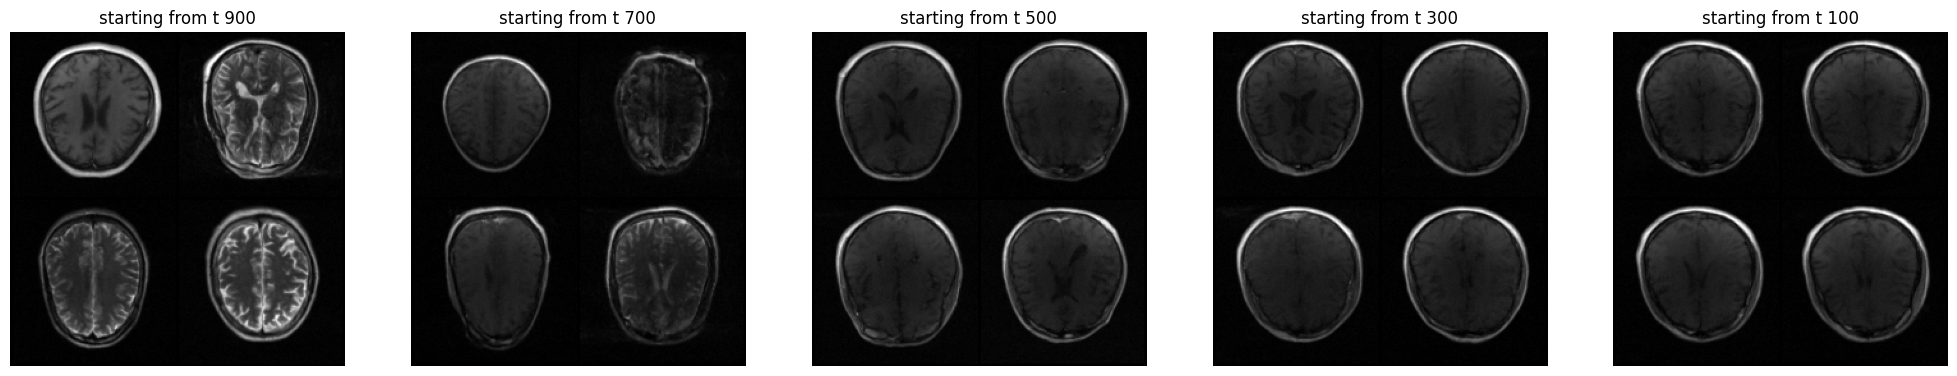
\includegraphics[width=.75\textwidth]{images/fixedlatents_variance.png}
    \caption[Variance in Predictions from Fixed Latents]{Variance in Predictions from Fixed Latents: The general shape of the final samples is already determined at $t=500$ and from there, the variability in the outputs is mostly about details of the structure.}
    \label{fig:predvariance}
\end{figure}
Variability in the samples can additionally be analyzed by inspecting the frequencies that carry most variance among the predictions. Those variances can be seen in Fig.~\ref{fig:spectralvariance} and while the variance is always concentrated in the center, as is expected from the spectrum of natural images, it can also be seen that the variance in the higher frequencies is proportionally higher at the end. This means that the information from higher frequencies matters much more towards the end, an observation that fits the SNR intuition from before.

\begin{figure}[h]
    \centering
    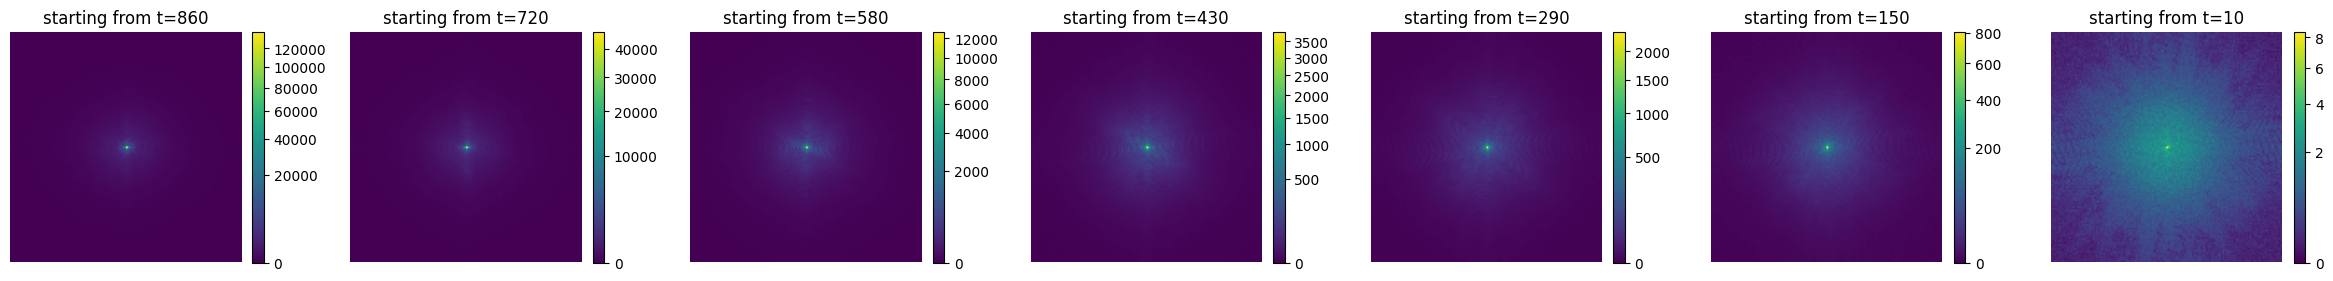
\includegraphics[width=\textwidth]{images/fixedlatents_varSpectra.png}
    \caption[Spectral Variance from Fixed Latents]{Variance in the Spectra when starting from Fixed Latents: When generating samples from fixed latent representation early in the denoising process, the variance of the spatial frequencies is highly concentrated in the center (e.g. $t=860$), overpowering the variance in the low frequencies by several orders of magnitude. The differences are smaller when starting late in the process (e.g. $t=10$), suggesting that fine details are only reconstructed at the very end. This hypothesis is also supported by the fact that natural images have lower SNR in the higher frequencies, which means that Gaussian perturbation affects them more and they can't carry much information until most of the noise is removed.}
    \label{fig:spectralvariance}
\end{figure}

In order to avoid a frequency mismatch during the reverse diffusion it could therefore make sense to add filtered k-space information, with gradually increasing passband over the reverse diffusion process, which could be done by introducing a schedule of standard deviations for the Gaussian kernel $\phi \rightarrow \phi(t)$ and applying it, in addition to the masking operation.
\begin{equation}
    x_{t-1} = x_t - \mathcal{F}^{-1}\left(\phi(t)\circ\mathcal{M}\circ\mathcal{F}(x_t) + \phi(t)\circ\mathcal{M}(s_t)\right)
\end{equation}
Results of such scheduled filters were in general unsatisfying with some samples showing a slight improvement in contrast, while aliasing was even amplified in others, as demonstrated in Fig.~\ref{fig:filtereddiffusion}. The search space over different schedules that could improve the outcome is very large and since loss guidance (\ref{sec:lossguidance}) had been identified as a very flexible and powerful approach at this point, optimization of the scheduling or resampling strategies using filter schedules were not further investigated. Loss guidance though offered another possibility of inspecting dominant frequencies in the guidance process and the results of this experiment are shown in Fig.~\ref{fig:lossgradients}.
\begin{figure}
    \centering
    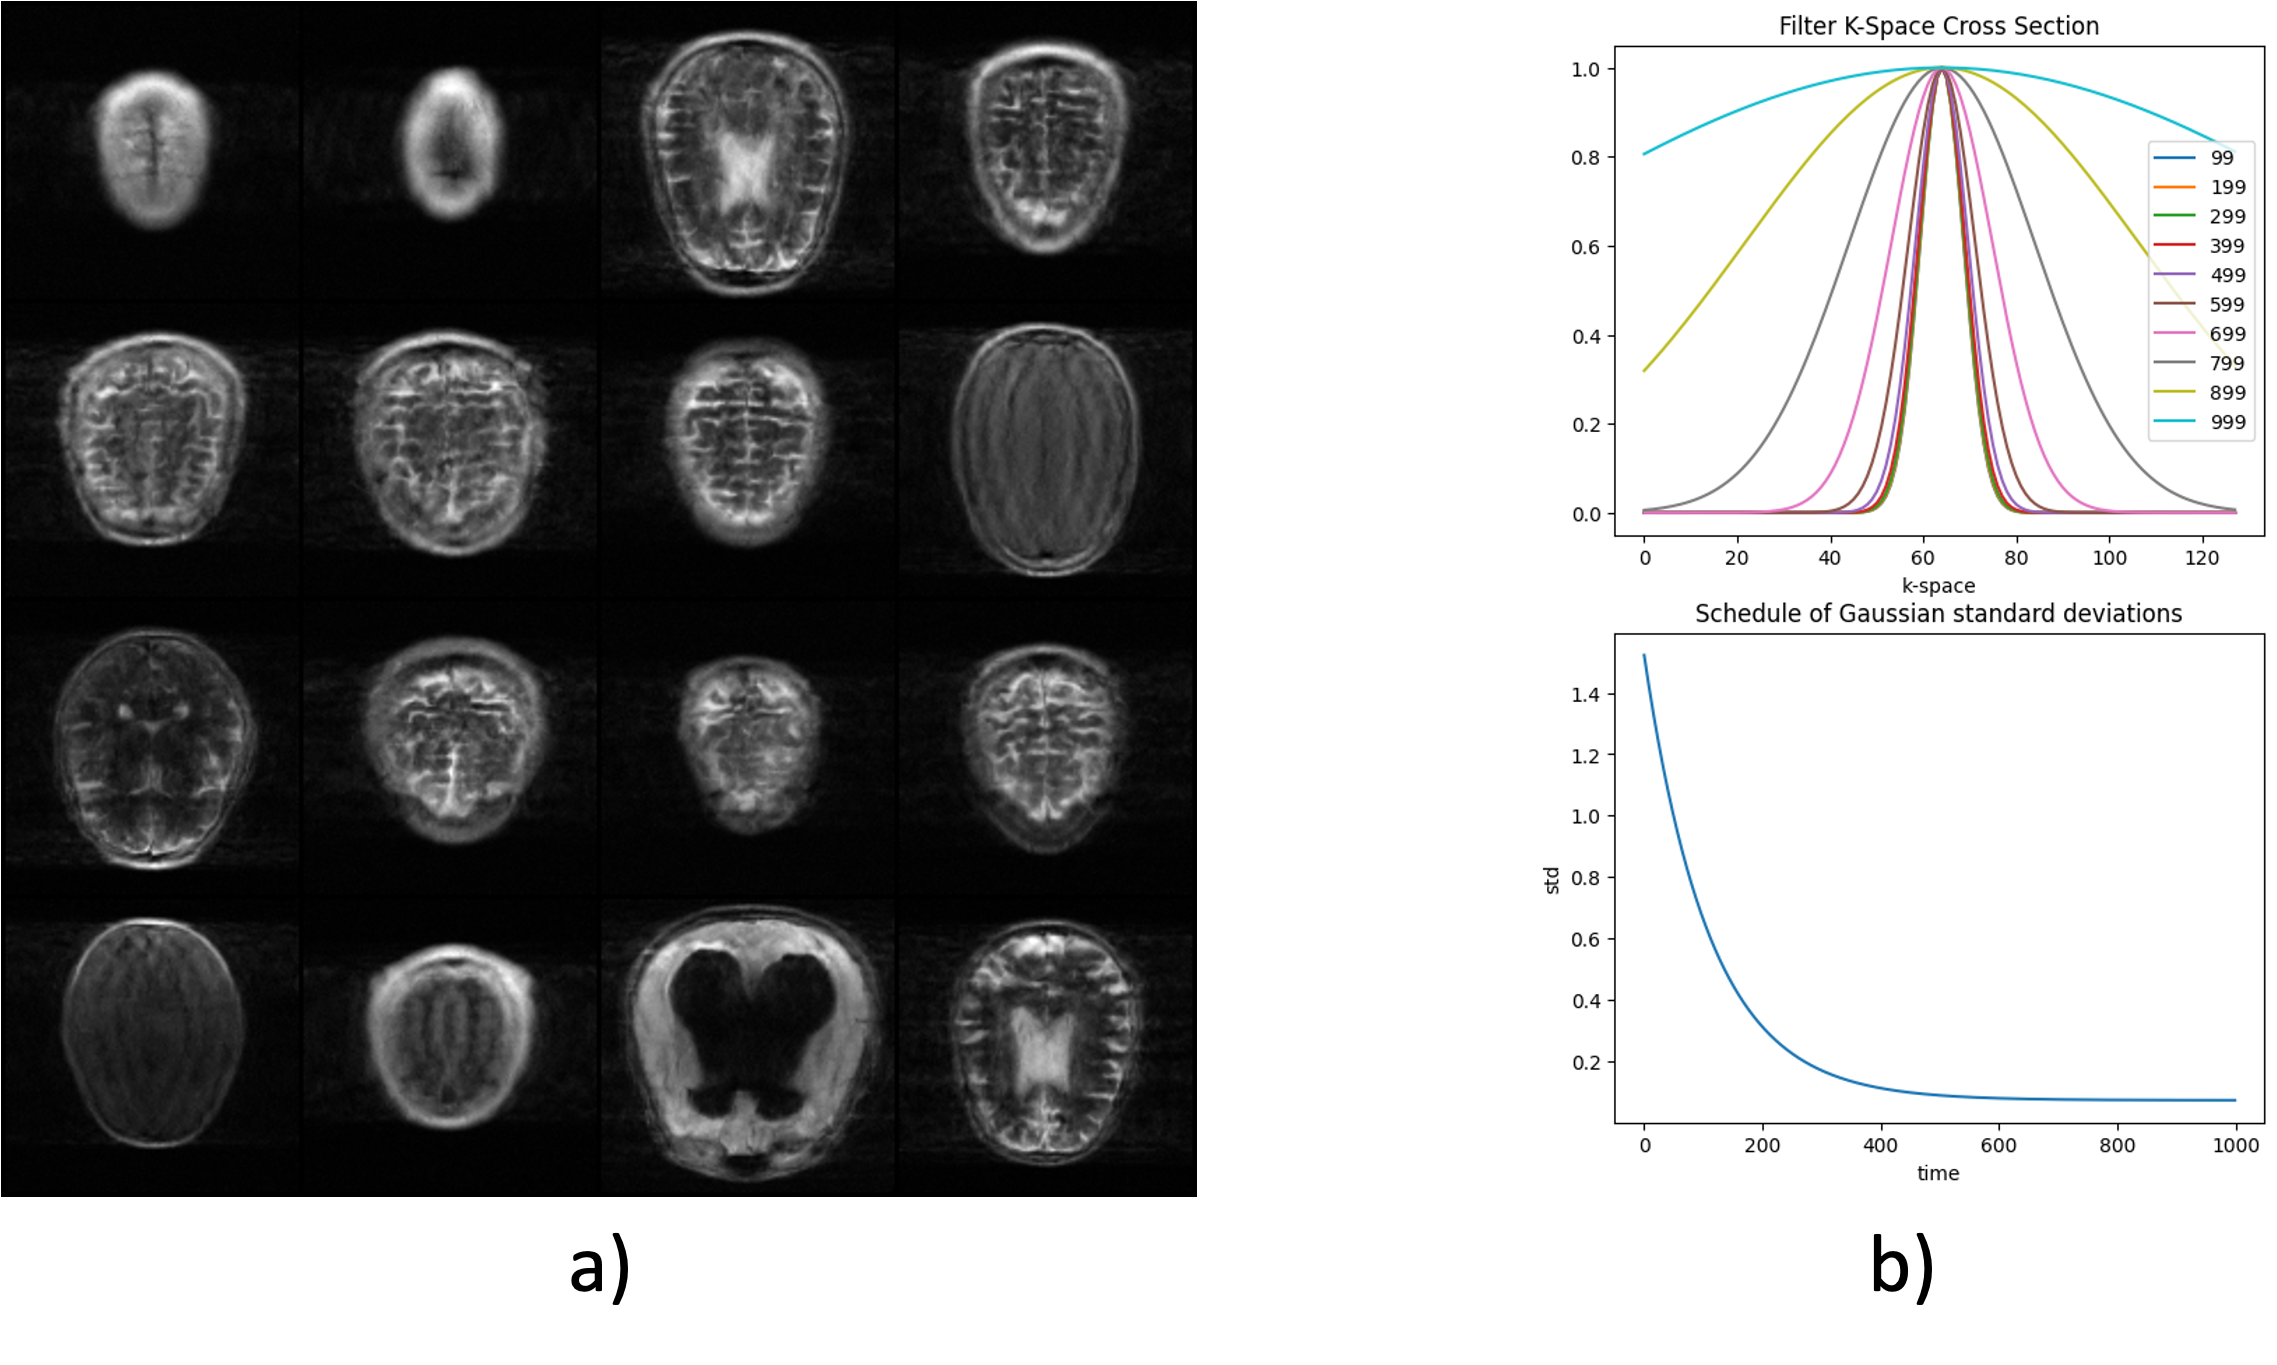
\includegraphics[width=.5\textwidth]{images/filtereddiffusion.png}
    \caption[short]{Results from scheduled filtering: a) Results from using Gaussian filters during reverse diffusion, scheduled according to the standard deviations in b) (lower). While contrast is in general enhanced compared to simple frequency replacement and some samples have better perceptual quality than before, aliasing seems amplified compared to before. While this was not further investigated, it may be that those samples were initially guided into a wrong distributional mode in which later introduced frequencies matched even worse.}
    \label{fig:filtereddiffusion}
\end{figure}

\section{Loss Function Guidance}
Taking gradient steps in the direction of a loss gradient immediately proved to be a more flexible approach with much better reconstruction results than the previous methods.
\begin{lstlisting}[language=iPython, caption=My Caption will come here., float=htbp, label=lst:labsetuptomo]
    import torch
\end{lstlisting}

\begin{figure}[h]
    \centering
    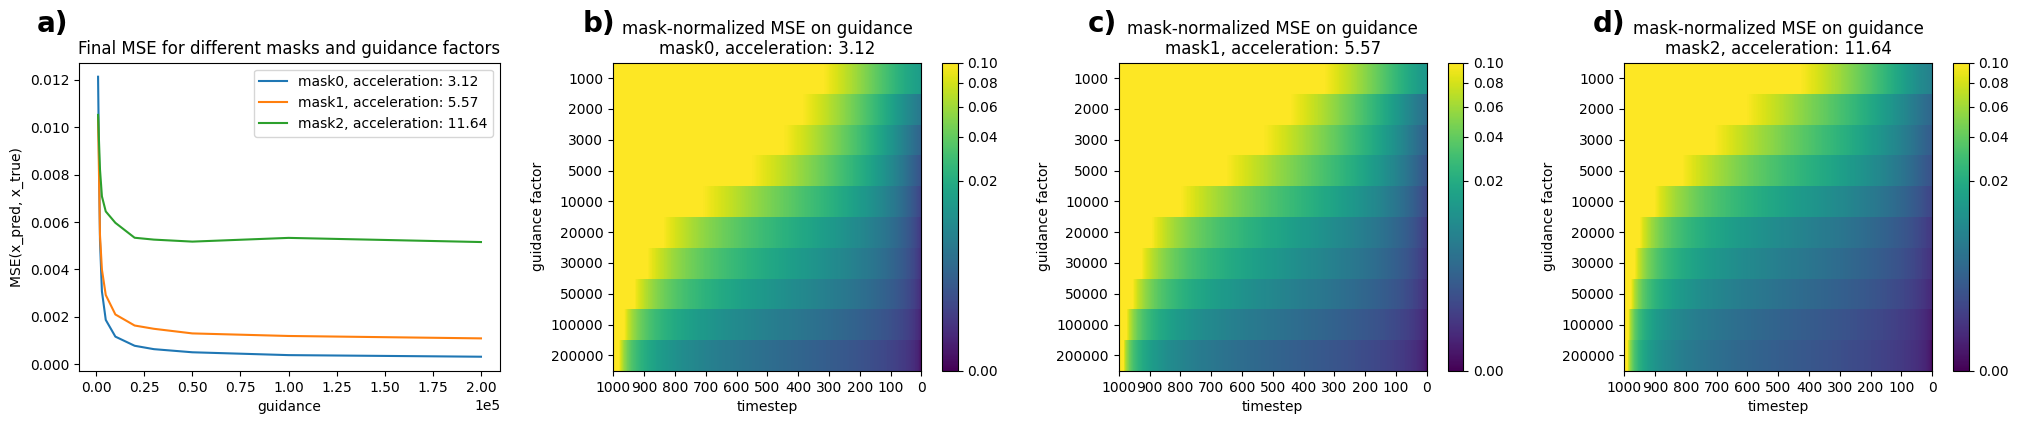
\includegraphics[width=\textwidth]{images/direct_sampling.png}
    \caption[Direct Sampling with Loss Guidance]{Results from Direct Sampling with Loss Guidance.}
\end{figure}